%%%%%%%%%%%%%%%%%%%%%%%%%%%%%%%%%%%%%%%%%
% Beamer Presentation
% LaTeX Template
% Version 1.0 (10/11/12)
%
% This template has been downloaded from:
% http://www.LaTeXTemplates.com
%
% License:
% CC BY-NC-SA 3.0 (http://creativecommons.org/licenses/by-nc-sa/3.0/)
%
%%%%%%%%%%%%%%%%%%%%%%%%%%%%%%%%%%%%%%%%%

%----------------------------------------------------------------------------------------
%	PACKAGES AND THEMES
%----------------------------------------------------------------------------------------

\documentclass{beamer}

\mode<presentation> {

% The Beamer class comes with a number of default slide themes
% which change the colors and layouts of slides. Below this is a list
% of all the themes, uncomment each in turn to see what they look like.

%\usetheme{default}
%\usetheme{AnnArbor}
%\usetheme{Antibes}
%\usetheme{Bergen}
%\usetheme{Berkeley}
%\usetheme{Berlin}
\usetheme{Boadilla}
%\usetheme{CambridgeUS}
%\usetheme{Copenhagen}
%\usetheme{Darmstadt}
%\usetheme{Dresden}
%\usetheme{Frankfurt}
%\usetheme{Goettingen}
%\usetheme{Hannover}
%\usetheme{Ilmenau}
%\usetheme{JuanLesPins}
%\usetheme{Luebeck}
%usetheme{Madrid}
%\usetheme{Malmoe}
%\usetheme{Marburg}
%\usetheme{Montpellier}
%usetheme{PaloAlto}
%\usetheme{Pittsburgh}
%\usetheme{Rochester}
%\usetheme{Singapore}
%\usetheme{Szeged}
%\usetheme{Warsaw}

% As well as themes, the Beamer class has a number of color themes
% for any slide theme. Uncomment each of these in turn to see how it
% changes the colors of your current slide theme.

%\usecolortheme{albatross}
%\usecolortheme{beaver}
%\usecolortheme{beetle}
%\usecolortheme{crane}
%\usecolortheme{dolphin}
%\usecolortheme{dove}
%\usecolortheme{fly}
%\usecolortheme{lily}
%\usecolortheme{orchid}
%\usecolortheme{rose}
%\usecolortheme{seagull}
%\usecolortheme{seahorse}
%\usecolortheme{whale}
%\usecolortheme{wolverine}

%\setbeamertemplate{footline} % To remove the footer line in all slides uncomment this line
%\setbeamertemplate{footline}[page number] % To replace the footer line in all slides with a simple slide count uncomment this line

%\setbeamertemplate{navigation symbols}{} % To remove the navigation symbols from the bottom of all slides uncomment this line
}

\usepackage{graphicx} % Allows including images
\usepackage{booktabs} % Allows the use of \toprule, \midrule and \bottomrule in tables

%----------------------------------------------------------------------------------------
%	TITLE PAGE
%----------------------------------------------------------------------------------------

\title[Feedback Modality]{Feedback Modality for Motor Imagery} % The short title appears at the bottom of every slide, the full title is only on the title page

\author{Michael Jaquier, Loic Jeanningros} % Your name
\institute[EPFL] % Your institution as it will appear on the bottom of every slide, may be shorthand to save space
{
EPFL \\ % Your institution for the title page
%\medskip
%\textit{john@smith.com} % Your email address
}
%\date{\today} % Date, can be changed to a custom date

\begin{document}

\begin{frame}
\titlepage % Print the title page as the first slide
\end{frame}


%----------------------------------------------------------------------------------------
%	PRESENTATION SLIDES
%----------------------------------------------------------------------------------------

%------------------------------------------------
%\section{Functional Electrical Stimulation (FES)} % Sections can be created in order to organize your presentation into discrete blocks, all sections and subsections are automatically printed in the table of contents as an overview of the talk
%------------------------------------------------

%\subsection{Low energy electrical stimulation utilized in to simulate normal motor action (e.x.\ grasping).} % A subsection can be created just before a set of slides with a common theme to further break down your presentation into chunks
\begin{frame}
	\frametitle{Feedback Modalities}
	\begin{figure}
		\includegraphics[width=0.55\linewidth]{fig/fespic}
	\end{figure}
	\textbf{Functional Electrical Stimulation:} Low energy electrical stimulation utilized in to simulate normal motor action (e.x.\ grasping).
\end{frame}

%------------------------------------------------

\begin{frame}
\frametitle{Protocol}
\begin{figure}
\includegraphics[width=0.8\linewidth]{fig/protocol}
\end{figure}
\begin{itemize}
\item \textbf{Fixation}: User focuses on cross on screen
\item \textbf{Cue}: User informed of required action (Rest/MI)
\item \textbf{Continuous Feedback}: User receives visual or electrical feedback
\item \textbf{Decision}: Arrow reaches top (visual). Muscle contraction (FES)
\item \textbf{Pause}: User allowed to adjust position, blink, etc. 
\end{itemize}
\end{frame}

%------------------------------------------------

\begin{frame}
\frametitle{EEG Recording}
\begin{figure}
	\includegraphics[width=0.8\linewidth]{fig/EEG}
\end{figure}
\begin{itemize}
\item Record from 64 electrodes, analysis on 16.
\item Remove NaN and noisy channels
\end{itemize}
\end{frame}

%------------------------------------------------

\begin{frame}
	\frametitle{Filtering}
	\begin{figure}
		\includegraphics[width=0.8\linewidth]{fig/filter}
	\end{figure}
	We attempted both common average reference (CAR) and small laplacian on both subjects. Our results suggest that the small laplacian filter was more effective on subject 2, whereas CAR proved best for subject 3. \cite{e1}
\end{frame}
%------------------------------------------------

\begin{frame}
\frametitle{pwelch - Visualization of ERD}
%\begin{columns}[c] % The "c" option specifies centered vertical alignment while the "t" option is used for top vertical alignment

%\column{.45\textwidth} % Left column and width
\textbf{pwelch parameters}
\begin{enumerate}
\item \textbf{Window Size}: 1 sec \\(512 samples)
\item \textbf{Window Overlap}: 50$ \% $
\item \textbf{Frequency Band}: 0.5-45Hz
\end{enumerate}

%\column{.5\textwidth} % Right column and width
\begin{figure}
	\includegraphics[width=0.8\linewidth]{fig/S6_psdVIS.eps}
\end{figure}
%\end{columns}
\end{frame}

%------------------------------------------------
%\section{Second Section}
%------------------------------------------------

\begin{frame}
\frametitle{Feature Selection}
In order to select features we analyzes the data utilizing a combination of statistical methods: 
\begin{itemize}
	\item R-Squared \begin{equation}
	\rho(X,Y) = \frac{{\bf
			Cov}(X,Y)}{\sqrt{{\bf Var}(X){\bf Var}(Y)}}
	\label{eq:e3}
	\end{equation}
	\item Fisher Score \begin{equation}
	F_r = \frac{\sum_{i=1}^c n_i(\mu_i - \mu)^2}{\sum_{i=1}^c n_i \sigma_i^2}
	\label{eq:e4}
	\end{equation}
\end{itemize}
In addition we utilized both \emph{students t-test} and \emph{independent feature modeling}. After examining each method we found that fisher scoring \cite{p3} was optimal for both subjects data sets. \\

In order to select features which were logical we limited ourselves to the $\mu$ (7.5 - 12.5 Hz) or $\beta$ (16 - 31 Hz) bands due to a priori knowledge of their significance in the sensorimotor areas \cite{p1},\cite{p2}. \
\end{frame}
%------------------------------------------------

\begin{frame}
\frametitle{Feature Plotting}
\begin{figure}

	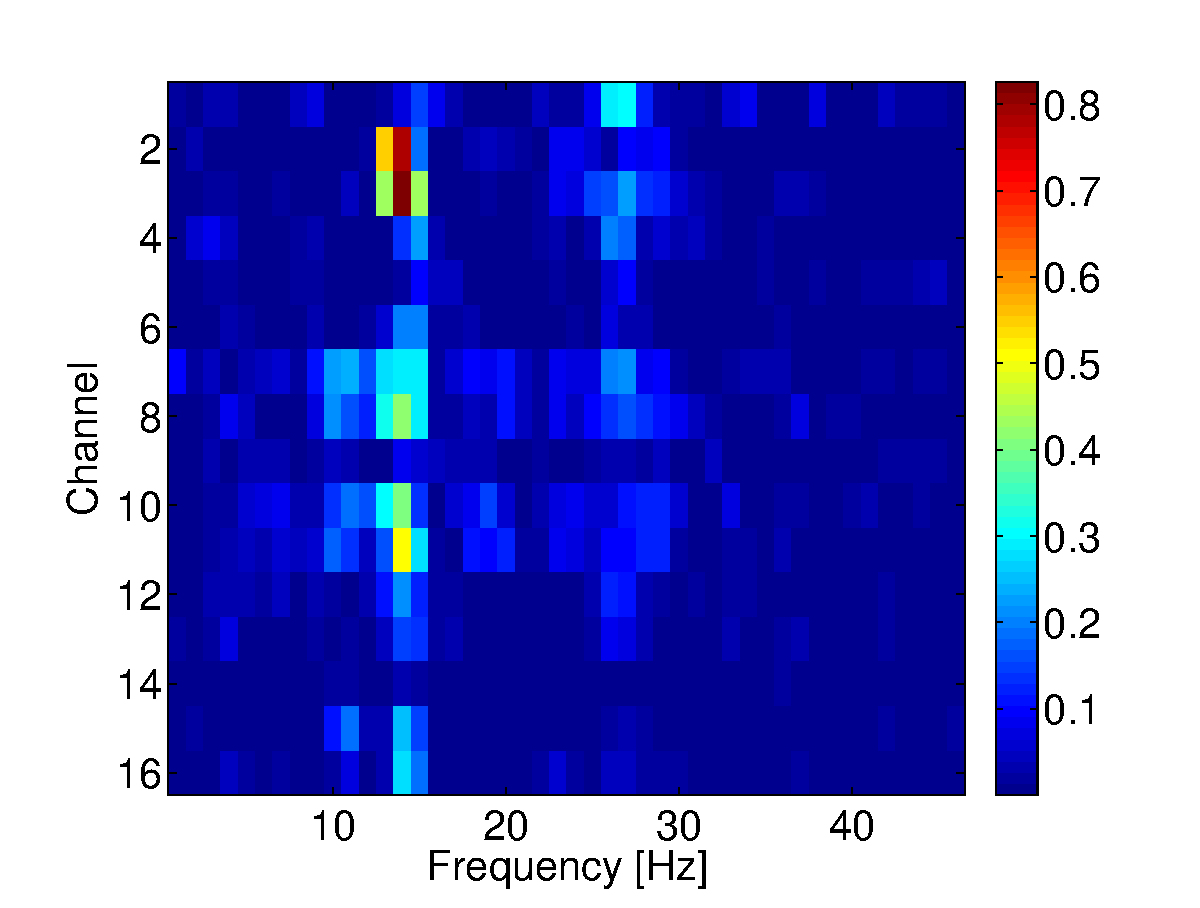
\includegraphics[width=0.45\linewidth]{fig/VISsession1.eps}
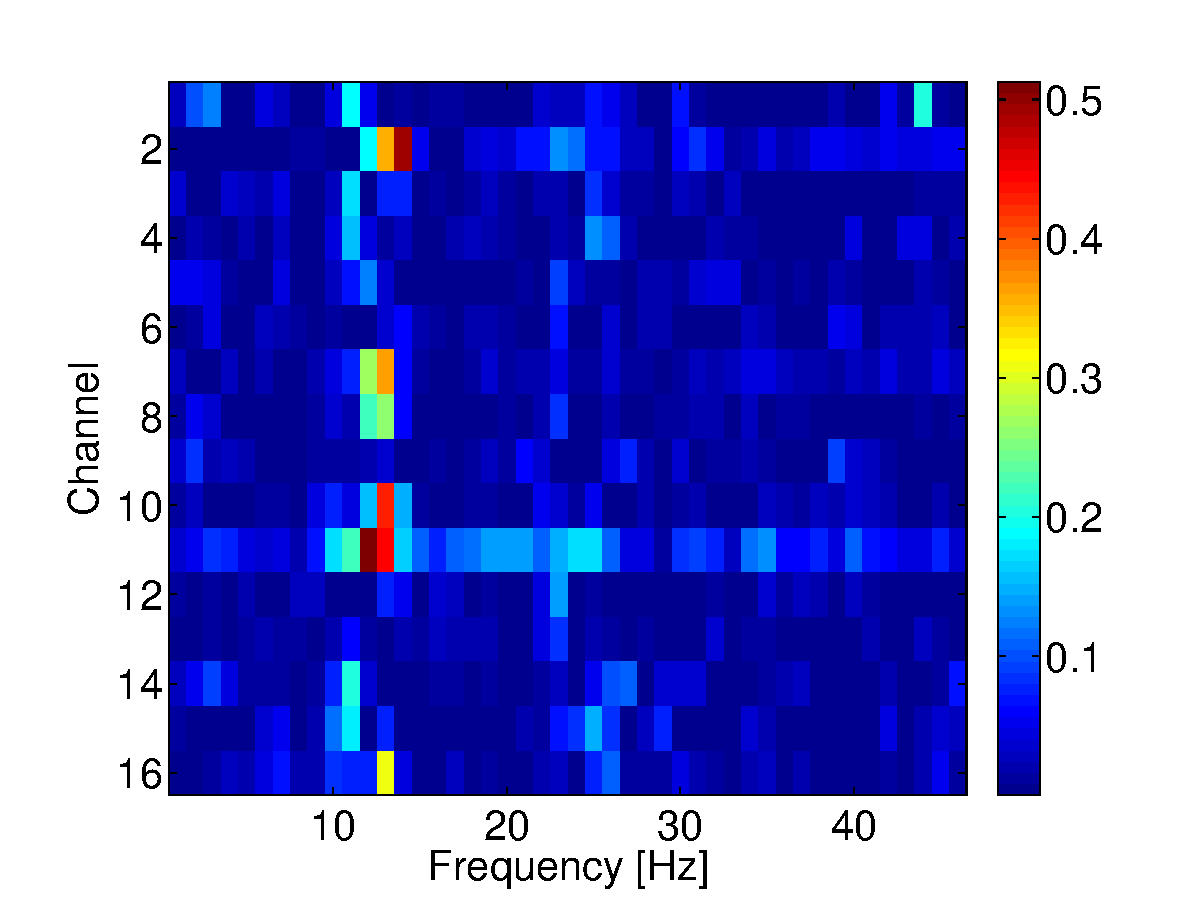
\includegraphics[width=0.45\linewidth]{fig/VISsession2.eps} 
\qquad
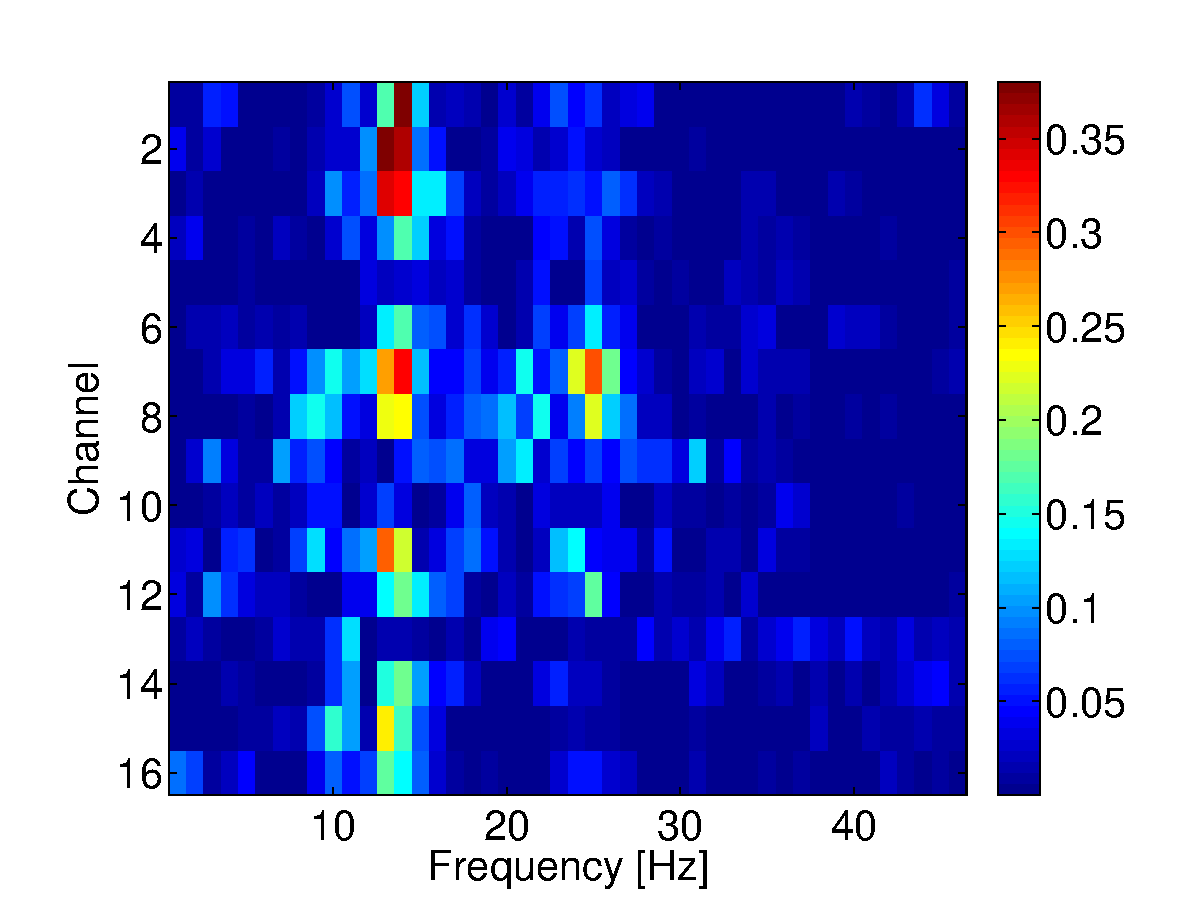
\includegraphics[width=0.45\linewidth]{fig/FESsession1.eps}
\includegraphics[width=0.45\linewidth]{fig/FESsession2.eps}
	\end{figure}
\end{frame}
%------------------------------------------------

\begin{frame} %[fragile] % Need to use the fragile option when verbatim is used in the slide
\frametitle{Topographic Feature Plotting}
\begin{figure}
	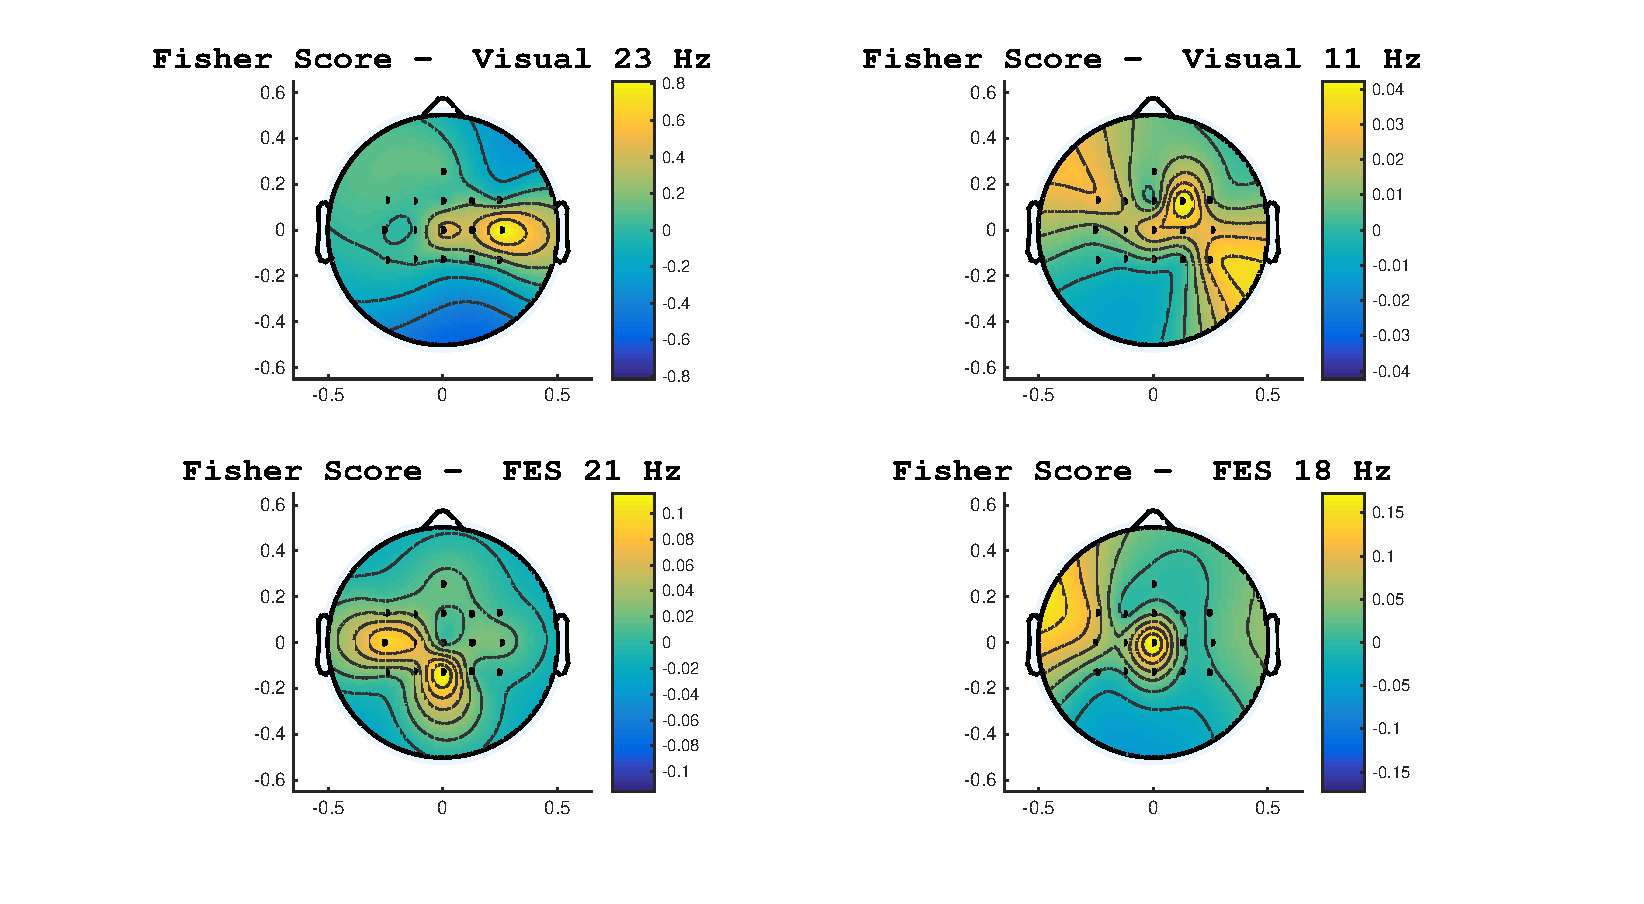
\includegraphics[width=0.95\linewidth]{fig/fishertopo.eps}
\end{figure}
\end{frame}

%------------------------------------------------

\begin{frame}
\frametitle{Classifiers }
\begin{figure}
	\includegraphics[width=0.75\linewidth]{fig/qdalda.png}
\end{figure}
[http://machine-learning-python.kspax.io]
%\begin{figure}
%\includegraphics[width=0.8\linewidth]{test}
%\end{figure}
\end{frame}

%------------------------------------------------

\begin{frame}%[fragile] % Need to use the fragile option when verbatim is used in the slide
\frametitle{Classifiers: Performance of QDA vs LDA}
\begin{figure}
	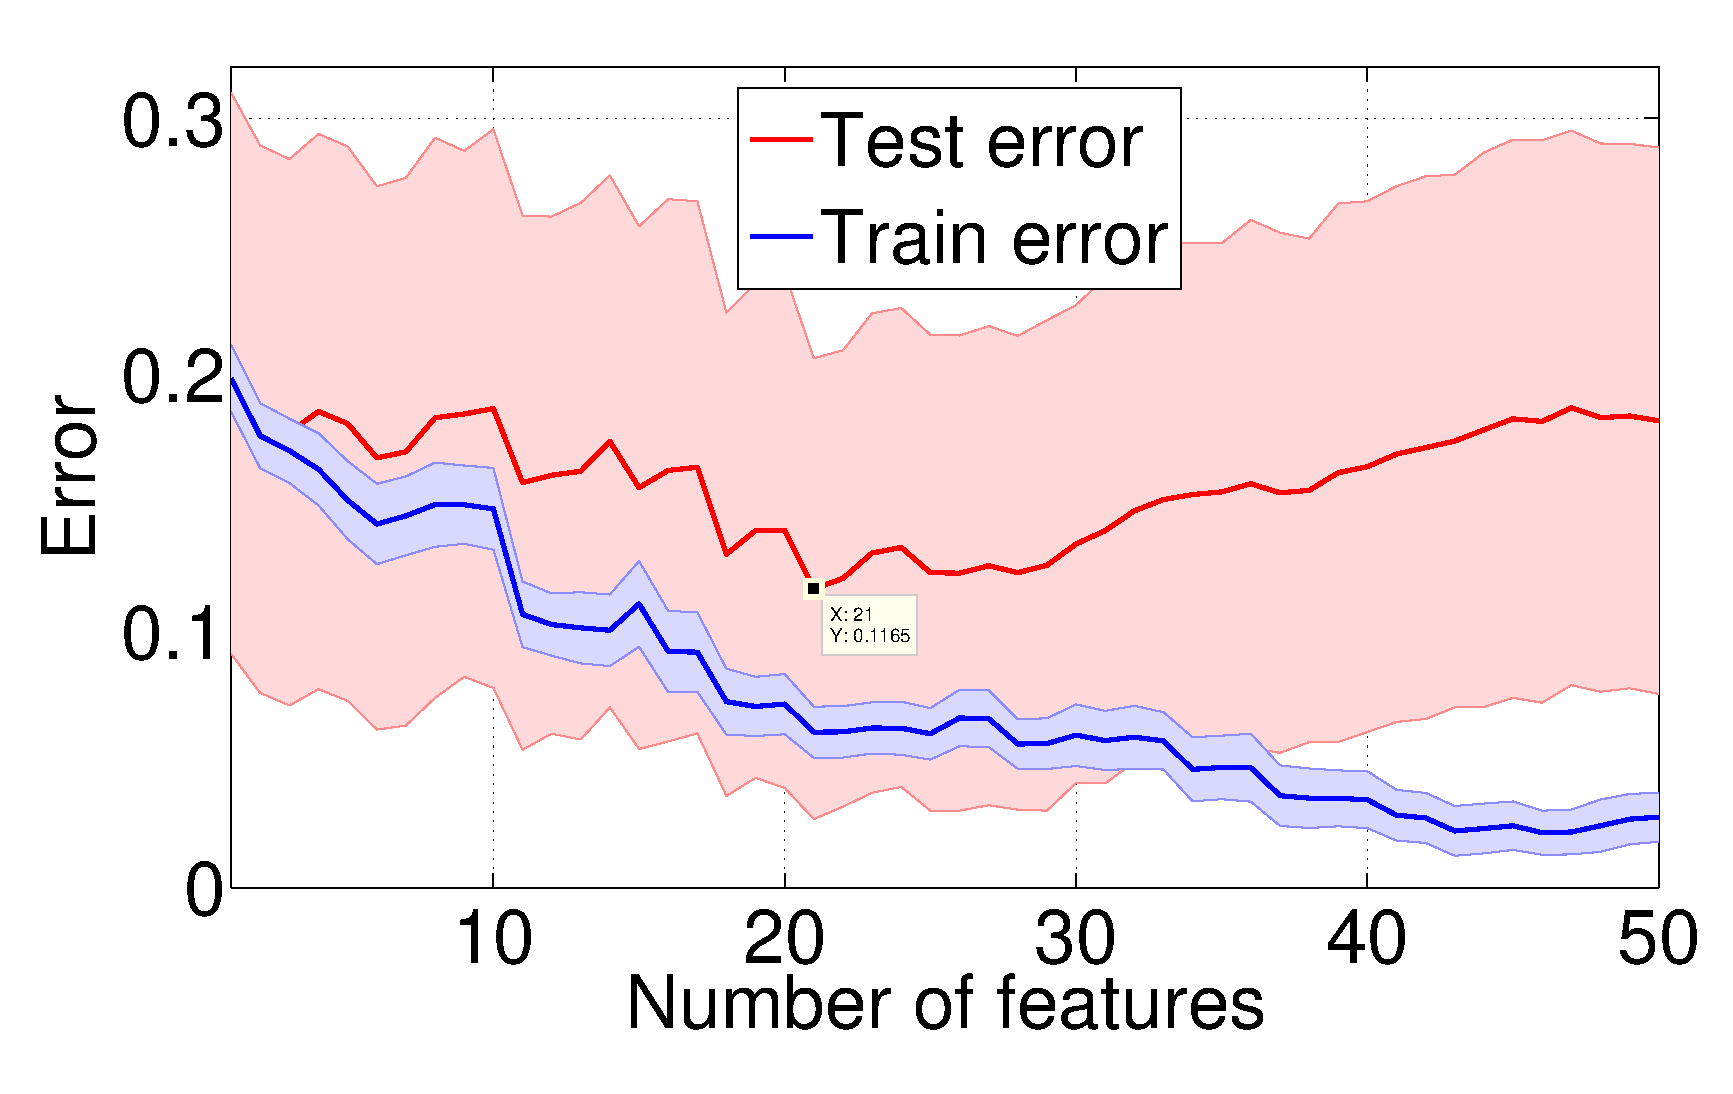
\includegraphics[width=0.45\linewidth]{fig/class_VIS_LDA.eps}
	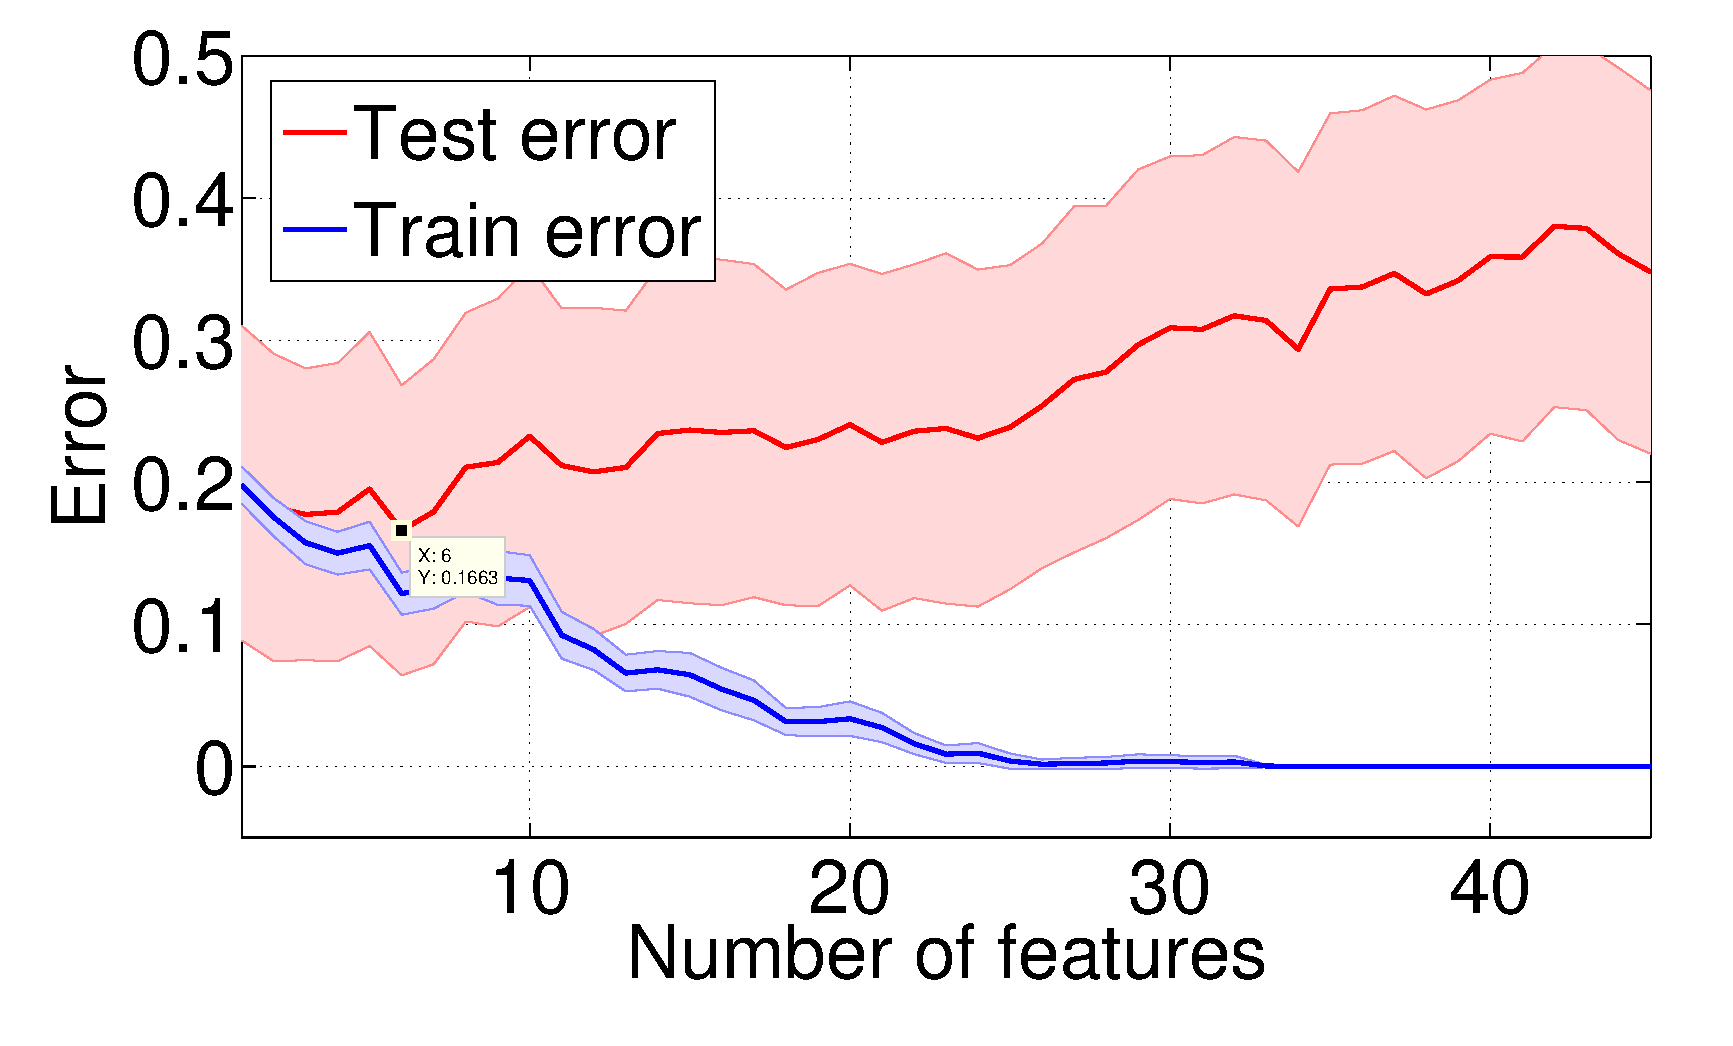
\includegraphics[width=0.45\linewidth]{fig/class_VIS_QDA.eps} 
	\qquad
		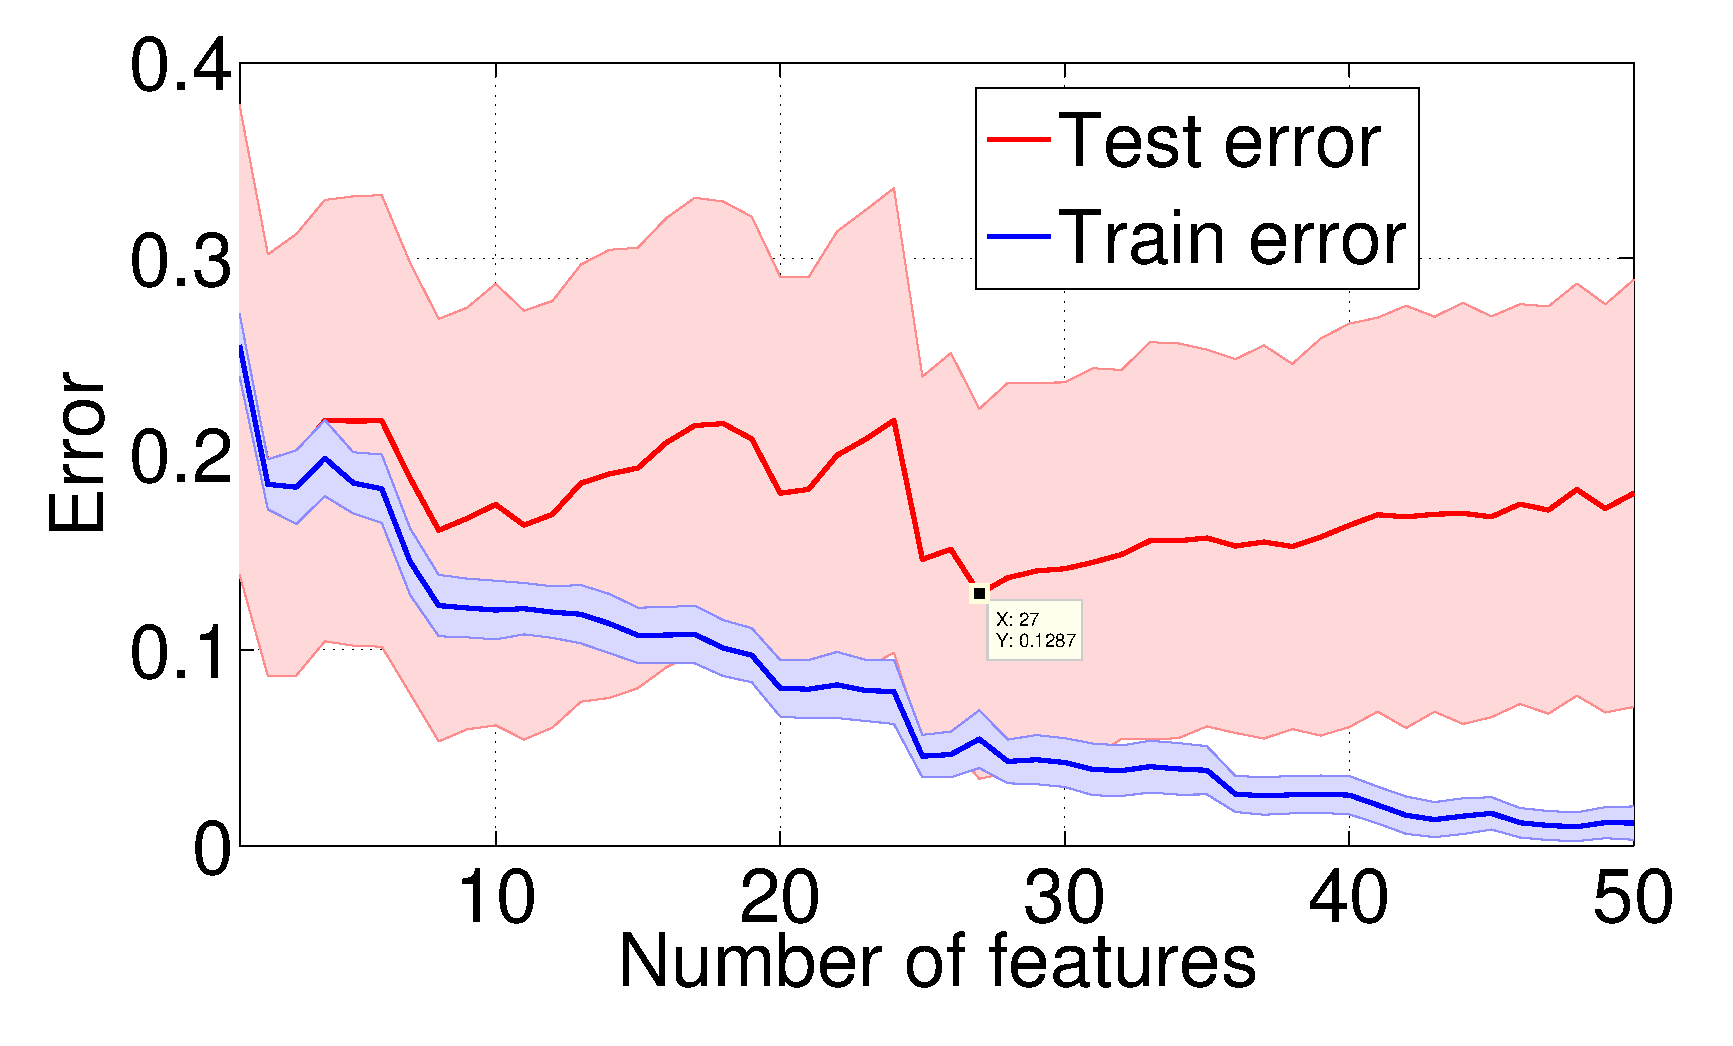
\includegraphics[width=0.45\linewidth]{fig/class_FES_LDA.eps}
		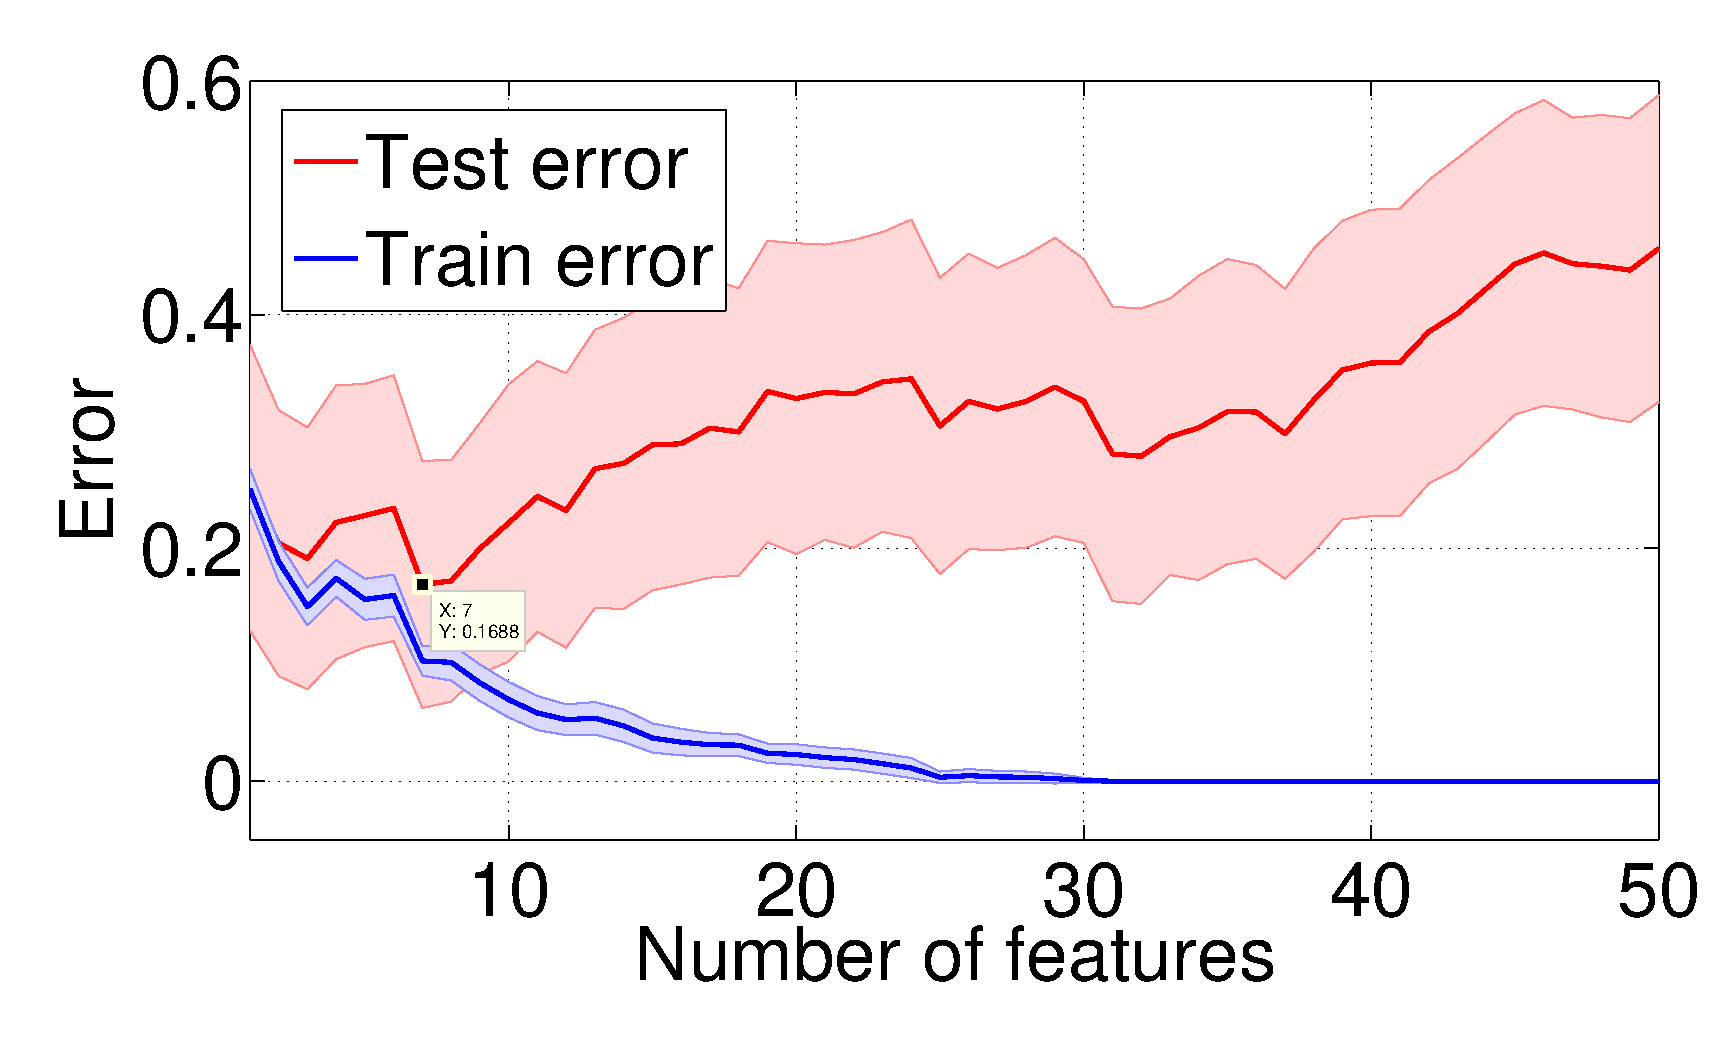
\includegraphics[width=0.45\linewidth]{fig/class_FES_QDA.eps}
\end{figure}
\end{frame}

%------------------------------------------------

\begin{frame}%[fragile] % Need to use the fragile option when verbatim is used in the slide
	\frametitle{FES: Control}
	\begin{figure}
		\includegraphics[width=0.75\linewidth]{fig/FeatSel_3.pdf}
	\end{figure}
\end{frame}

%------------------------------------------------

\begin{frame}%[fragile] % Need to use the fragile option when verbatim is used in the slide
	\frametitle{FES: Control}
	\begin{figure}
		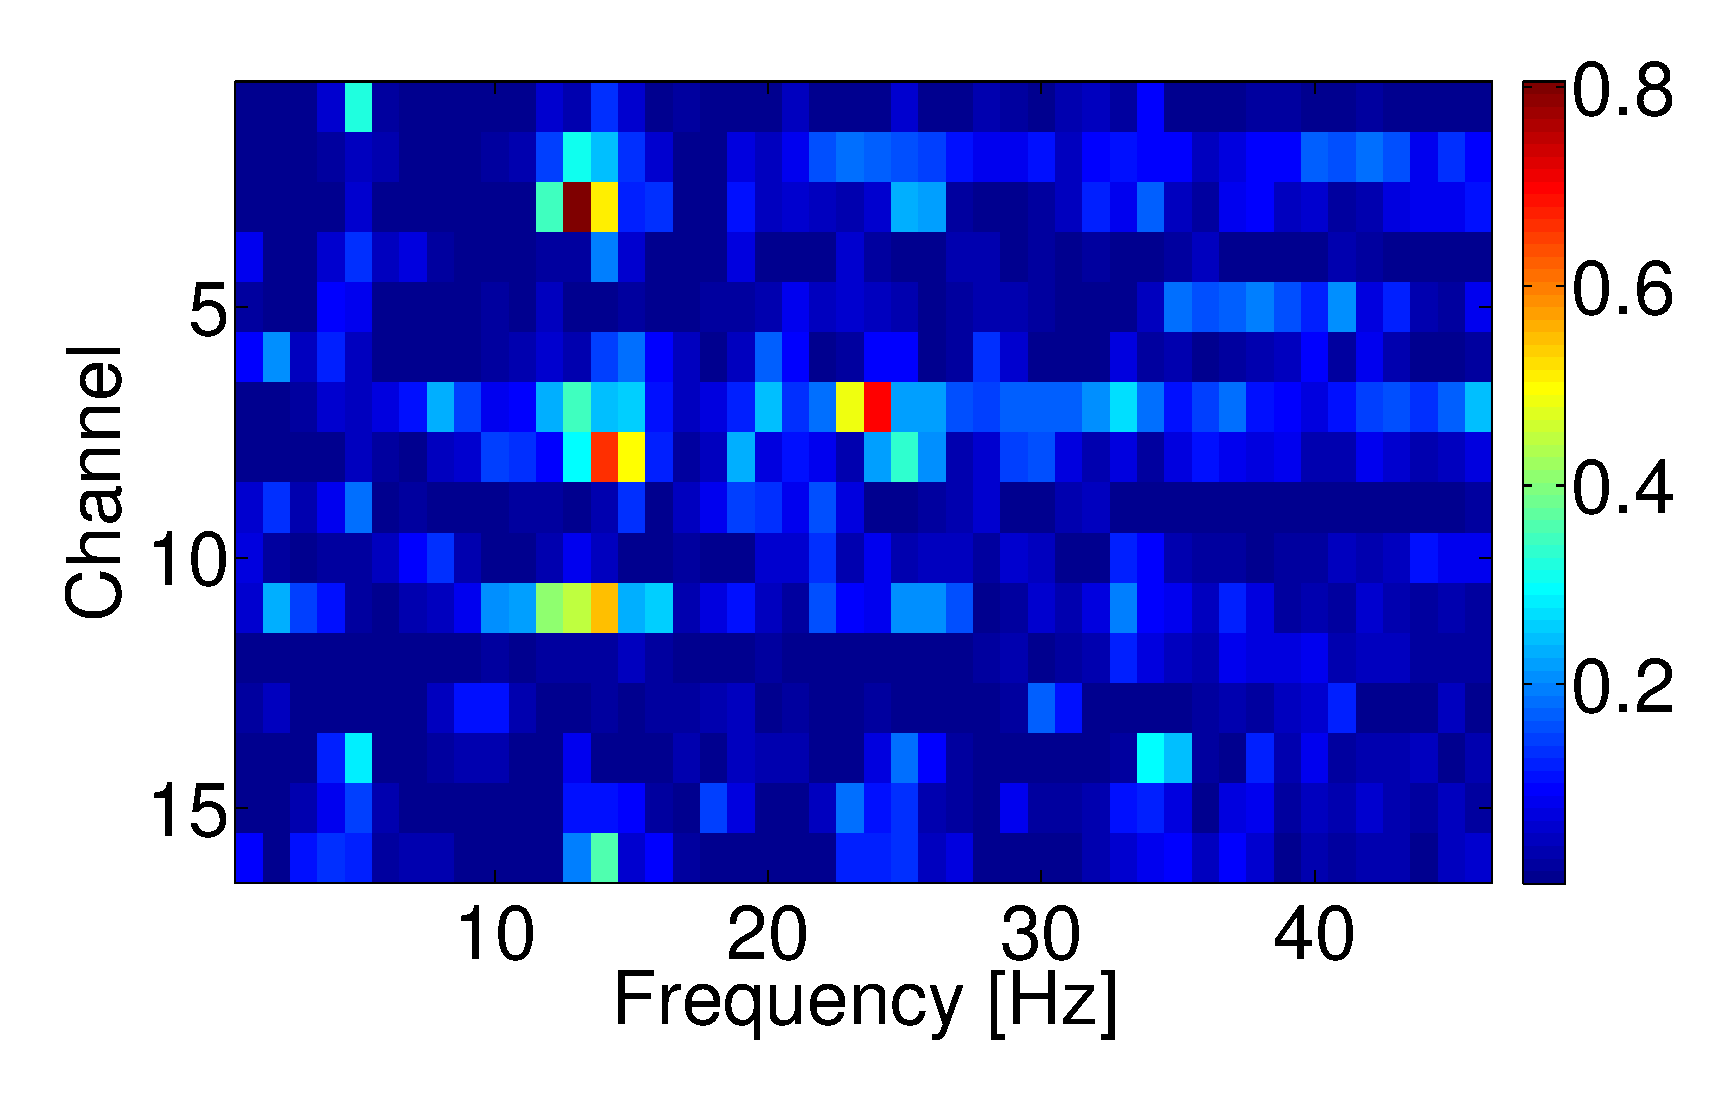
\includegraphics[width=0.75\linewidth]{fig/disc_FESnoMI.eps}
	\end{figure}
Fisher score of Subject 2's NoMI-FES control. Note that unlike the previous figure there are distinct features present here which overlap our features utilized for classification. 
\end{frame}

%------------------------------------------------
\begin{frame}%[fragile] % Need to use the fragile option when verbatim is used in the slide
	\frametitle{Results}
	\begin{figure}
		\includegraphics[width=0.50\linewidth]{fig/clasi.eps}
		\includegraphics[width=0.50\linewidth]{fig/clasi2.eps}
	\end{figure}
	Misclassification rates of LDA and QDA classifiers during session 1 for both FES and visual feedback for both subjects.
\end{frame}
%------------------------------------------------
\begin{frame}
\frametitle{References}
\footnotesize{
\begin{thebibliography}{99} % Beamer does not support BibTeX so references must be inserted manually as below
\bibitem[McFarland, 1997]{e1} McFarland DJ1, McCane LM, David SV, Wolpaw JR. (1997)
\newblock Spatial filter selection for EEG-based communication.
\newblock \emph{Electroencephalogr Clin Neurophysiol} 103(3):386-94.


\bibitem[Pfurtscheller, 2006]{p1} G. Pfurtscheller, C. Brunner, A. Schlo ̈gl, and F. H. Lopes da Silva (2016)
\newblock Mu rhythm (de)synchronization and eeg single-trial classification of different motor imagery tasks.
\newblock \emph{NeuroImagery} 31(1), 153–-159.
\bibitem[Pfurtscheller, 1997]{p2} Gert Pfurtscheller and Christa Neuper. (1997)
\newblock Motor imagery activates primary sensorimotor area in humans.
\newblock \emph{Neuroscience Letters} 239(2-3), 65–68, 12.
\bibitem[Xiaofei, 2005]{p3} Xiaofei He, Deng Cai, and Partha Niyogi (2005)
\newblock  Laplacian score for feature selection.
\newblock \emph{Advances in neural information processing systems} 507–514.
\end{thebibliography}
}
\end{frame}
%------------------------------------------------

\begin{frame}
\Huge{\centerline{Questions}}
\end{frame}

%----------------------------------------------------------------------------------------

\end{document} 